\documentclass[11pt]{article}
\usepackage[textwidth=18.0cm, textheight=23.0cm, top=2.0cm]{geometry}
\usepackage{pst-all}
\usepackage{amssymb}
\usepackage{tikz}
\usepackage{underscore}\begin{document}
\pagestyle{empty}


ClassName: \underline{\textbf{Class_03.2bp-10}}
\par
BinSize: \underline{\textbf{40 × 40}}
\par
ReduceSize: \underline{\textbf{40 × 40}}
\par
TypeNum: \underline{\textbf{39}}
\par
Num: \underline{\textbf{40}}
\par
OutS: \underline{\textbf{9600}}
\par
InS: \underline{\textbf{8968}}
\par
Rate: \underline{\textbf{0.934}}
\par
UB: \underline{\textbf{6}}
\par
LB0: \underline{\textbf{6}}
\par
LB: \underline{\textbf{6}}
\par
LBWithCut: \underline{\textbf{6}}
\par
NodeCut: \underline{\textbf{0}}
\par
ExtendedNodeCnt: \underline{\textbf{1}}
\par
GenNodeCnt: \underline{\textbf{1}}
\par
PrimalNode: \underline{\textbf{0}}
\par
ColumnCount: \underline{\textbf{6}}
\par
TotalCutCount: \underline{\textbf{0}}
\par
RootCutCount: \underline{\textbf{0}}
\par
LPSolverCnt: \underline{\textbf{1}}
\par
PricingSolverCnt: \underline{\textbf{0}}
\par
BranchAndBoundNum: \underline{\textbf{1}}
\par
isOpt: \underline{\textbf{true}}
\par
TimeOnInitSolution: \underline{\textbf{0.020 s}}
\par
TimeOnPrimal: \underline{\textbf{0.000 s}}
\par
TimeOnPricing: \underline{\textbf{0.000 s}}
\par
TimeOnRmp: \underline{\textbf{0.062 s}}
\par
TotalTime: \underline{\textbf{0.145 s}}
\par
\newpage


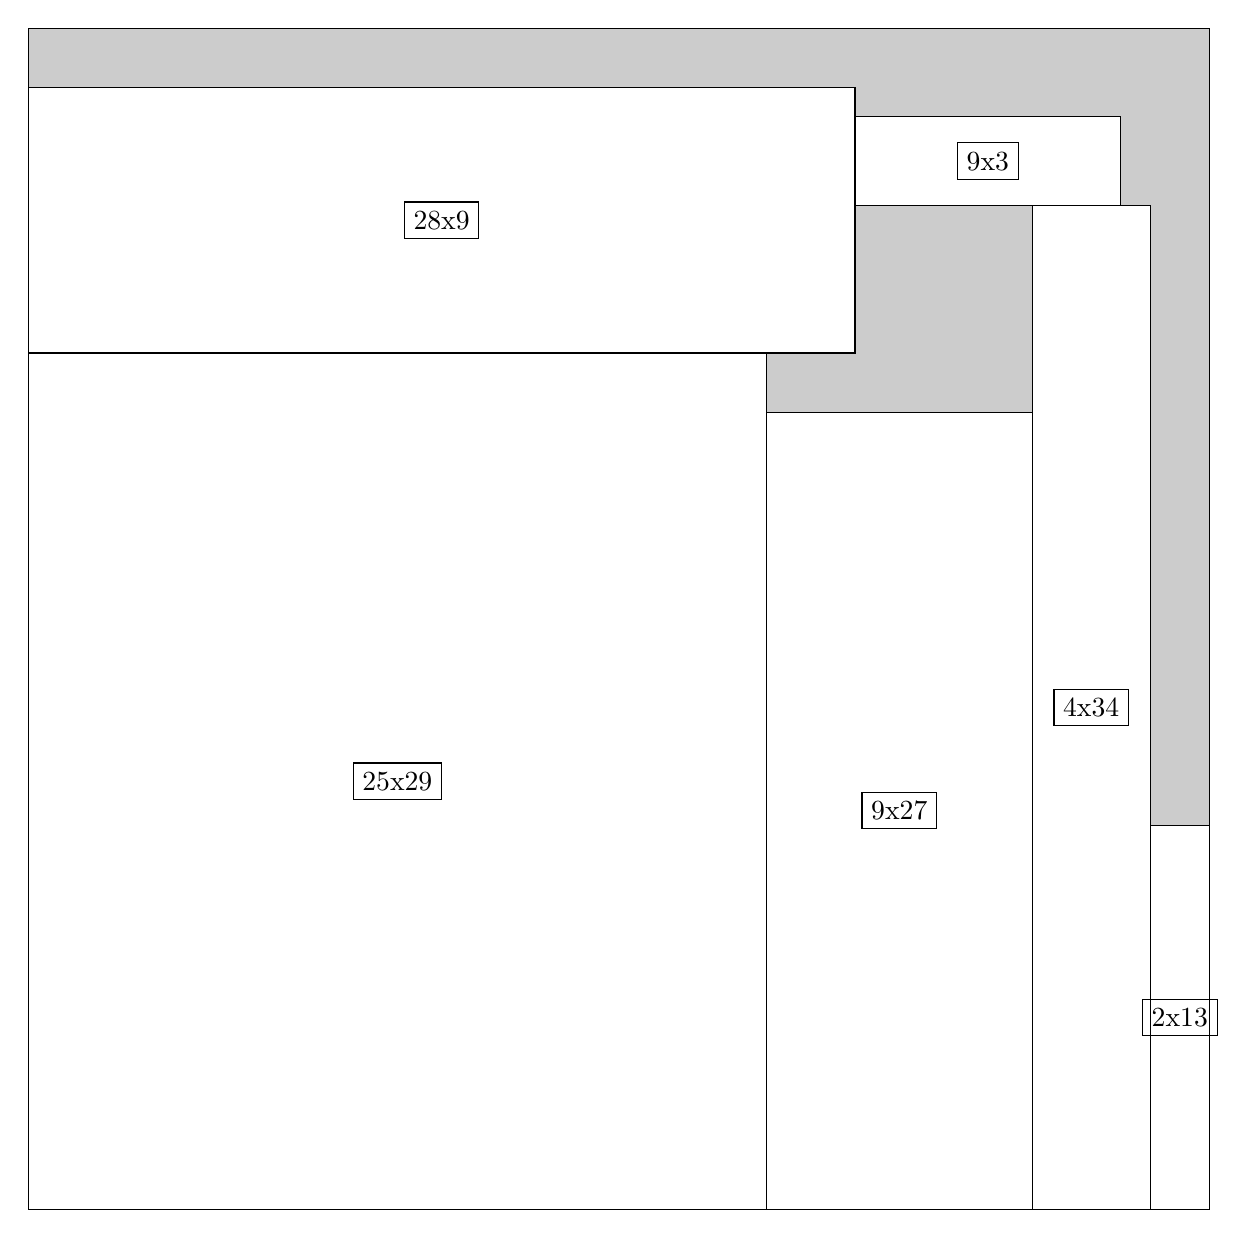
\begin{tikzpicture}[shorten >=1pt,scale=1.0,every node/.style={scale=1.0},->]
\tikzstyle{vertex}=[circle,fill=black!25,minimum size=14pt,inner sep=0pt]
\filldraw[fill=gray!40!white, draw=black] (0,0) rectangle (15.0,15.0);
\foreach \name/\x/\y/\w/\h in {25x29/0.0/0.0/9.375/10.875,28x9/0.0/10.875/10.5/3.375,9x27/9.375/0.0/3.375/10.125,4x34/12.75/0.0/1.5/12.75,9x3/10.5/12.75/3.375/1.125,2x13/14.25/0.0/0.75/4.875}
\filldraw[fill=white!40!white, draw=black] (\x,\y) rectangle node[draw] (\name) {\name} ++(\w,\h);
\end{tikzpicture}


w =25 , h =29 , x =0 , y =0 , v =725
\par
w =28 , h =9 , x =0 , y =29 , v =252
\par
w =9 , h =27 , x =25 , y =0 , v =243
\par
w =4 , h =34 , x =34 , y =0 , v =136
\par
w =9 , h =3 , x =28 , y =34 , v =27
\par
w =2 , h =13 , x =38 , y =0 , v =26
\par
\newpage


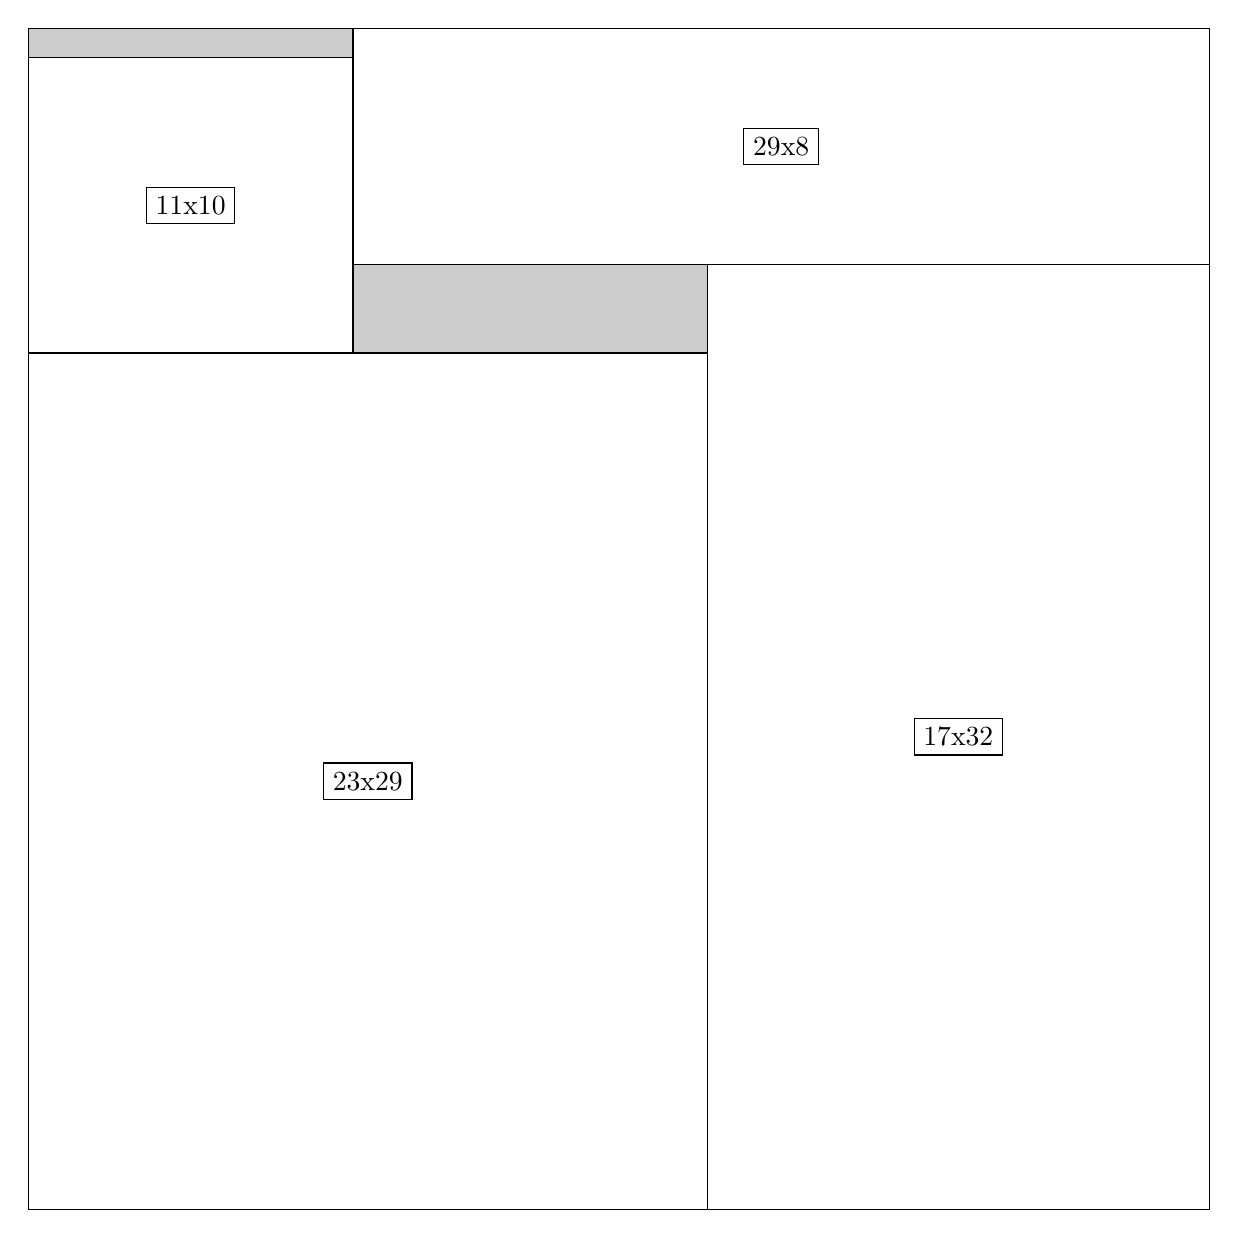
\begin{tikzpicture}[shorten >=1pt,scale=1.0,every node/.style={scale=1.0},->]
\tikzstyle{vertex}=[circle,fill=black!25,minimum size=14pt,inner sep=0pt]
\filldraw[fill=gray!40!white, draw=black] (0,0) rectangle (15.0,15.0);
\foreach \name/\x/\y/\w/\h in {17x32/8.625/0.0/6.375/12.0,23x29/0.0/0.0/8.625/10.875,29x8/4.125/12.0/10.875/3.0,11x10/0.0/10.875/4.125/3.75}
\filldraw[fill=white!40!white, draw=black] (\x,\y) rectangle node[draw] (\name) {\name} ++(\w,\h);
\end{tikzpicture}


w =17 , h =32 , x =23 , y =0 , v =544
\par
w =23 , h =29 , x =0 , y =0 , v =667
\par
w =29 , h =8 , x =11 , y =32 , v =232
\par
w =11 , h =10 , x =0 , y =29 , v =110
\par
\newpage


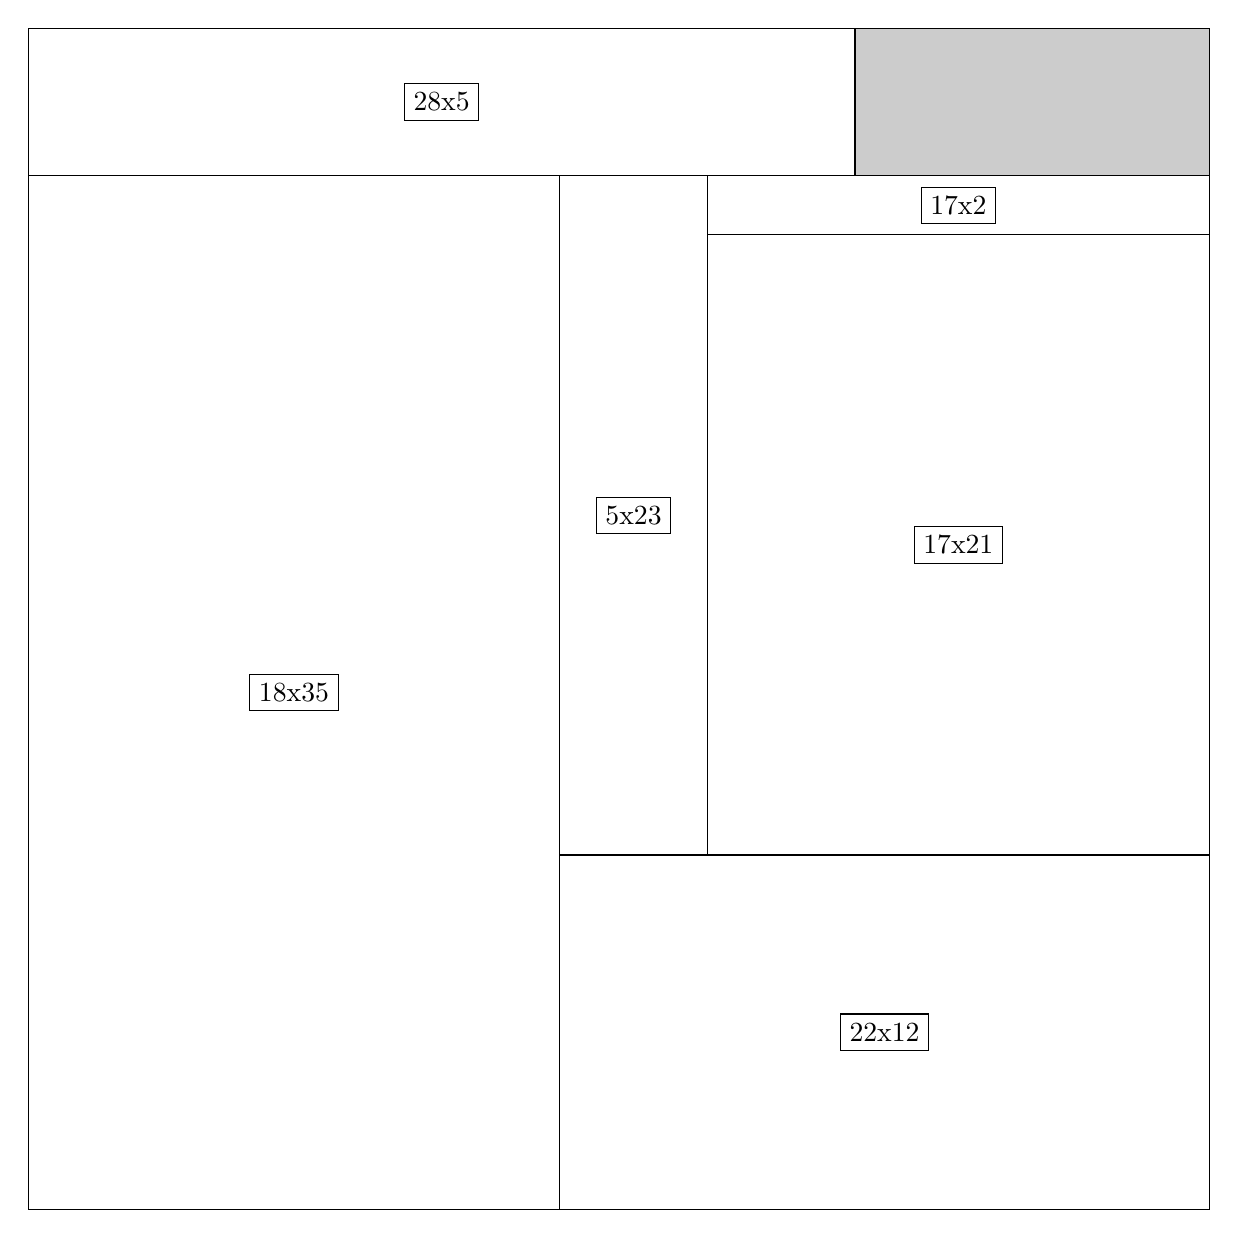
\begin{tikzpicture}[shorten >=1pt,scale=1.0,every node/.style={scale=1.0},->]
\tikzstyle{vertex}=[circle,fill=black!25,minimum size=14pt,inner sep=0pt]
\filldraw[fill=gray!40!white, draw=black] (0,0) rectangle (15.0,15.0);
\foreach \name/\x/\y/\w/\h in {18x35/0.0/0.0/6.75/13.125,17x21/8.625/4.5/6.375/7.875,22x12/6.75/0.0/8.25/4.5,28x5/0.0/13.125/10.5/1.875,5x23/6.75/4.5/1.875/8.625,17x2/8.625/12.375/6.375/0.75}
\filldraw[fill=white!40!white, draw=black] (\x,\y) rectangle node[draw] (\name) {\name} ++(\w,\h);
\end{tikzpicture}


w =18 , h =35 , x =0 , y =0 , v =630
\par
w =17 , h =21 , x =23 , y =12 , v =357
\par
w =22 , h =12 , x =18 , y =0 , v =264
\par
w =28 , h =5 , x =0 , y =35 , v =140
\par
w =5 , h =23 , x =18 , y =12 , v =115
\par
w =17 , h =2 , x =23 , y =33 , v =34
\par
\newpage


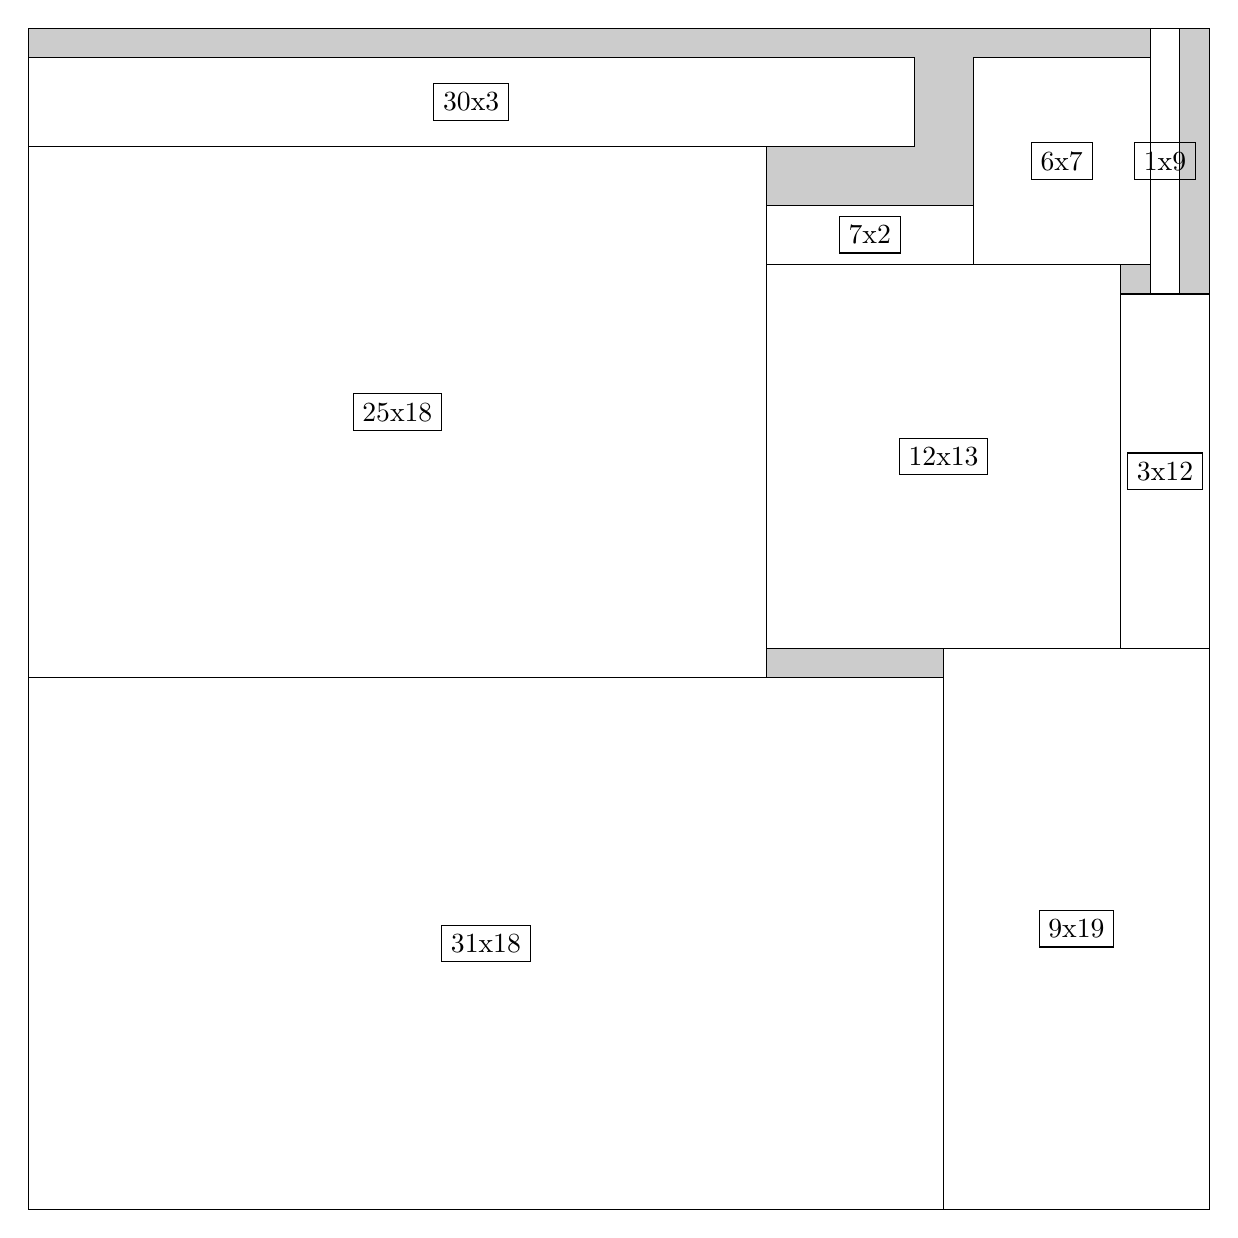
\begin{tikzpicture}[shorten >=1pt,scale=1.0,every node/.style={scale=1.0},->]
\tikzstyle{vertex}=[circle,fill=black!25,minimum size=14pt,inner sep=0pt]
\filldraw[fill=gray!40!white, draw=black] (0,0) rectangle (15.0,15.0);
\foreach \name/\x/\y/\w/\h in {31x18/0.0/0.0/11.625/6.75,25x18/0.0/6.75/9.375/6.75,9x19/11.625/0.0/3.375/7.125,12x13/9.375/7.125/4.5/4.875,30x3/0.0/13.5/11.25/1.125,6x7/12.0/12.0/2.25/2.625,3x12/13.875/7.125/1.125/4.5,7x2/9.375/12.0/2.625/0.75,1x9/14.25/11.625/0.375/3.375}
\filldraw[fill=white!40!white, draw=black] (\x,\y) rectangle node[draw] (\name) {\name} ++(\w,\h);
\end{tikzpicture}


w =31 , h =18 , x =0 , y =0 , v =558
\par
w =25 , h =18 , x =0 , y =18 , v =450
\par
w =9 , h =19 , x =31 , y =0 , v =171
\par
w =12 , h =13 , x =25 , y =19 , v =156
\par
w =30 , h =3 , x =0 , y =36 , v =90
\par
w =6 , h =7 , x =32 , y =32 , v =42
\par
w =3 , h =12 , x =37 , y =19 , v =36
\par
w =7 , h =2 , x =25 , y =32 , v =14
\par
w =1 , h =9 , x =38 , y =31 , v =9
\par
\newpage


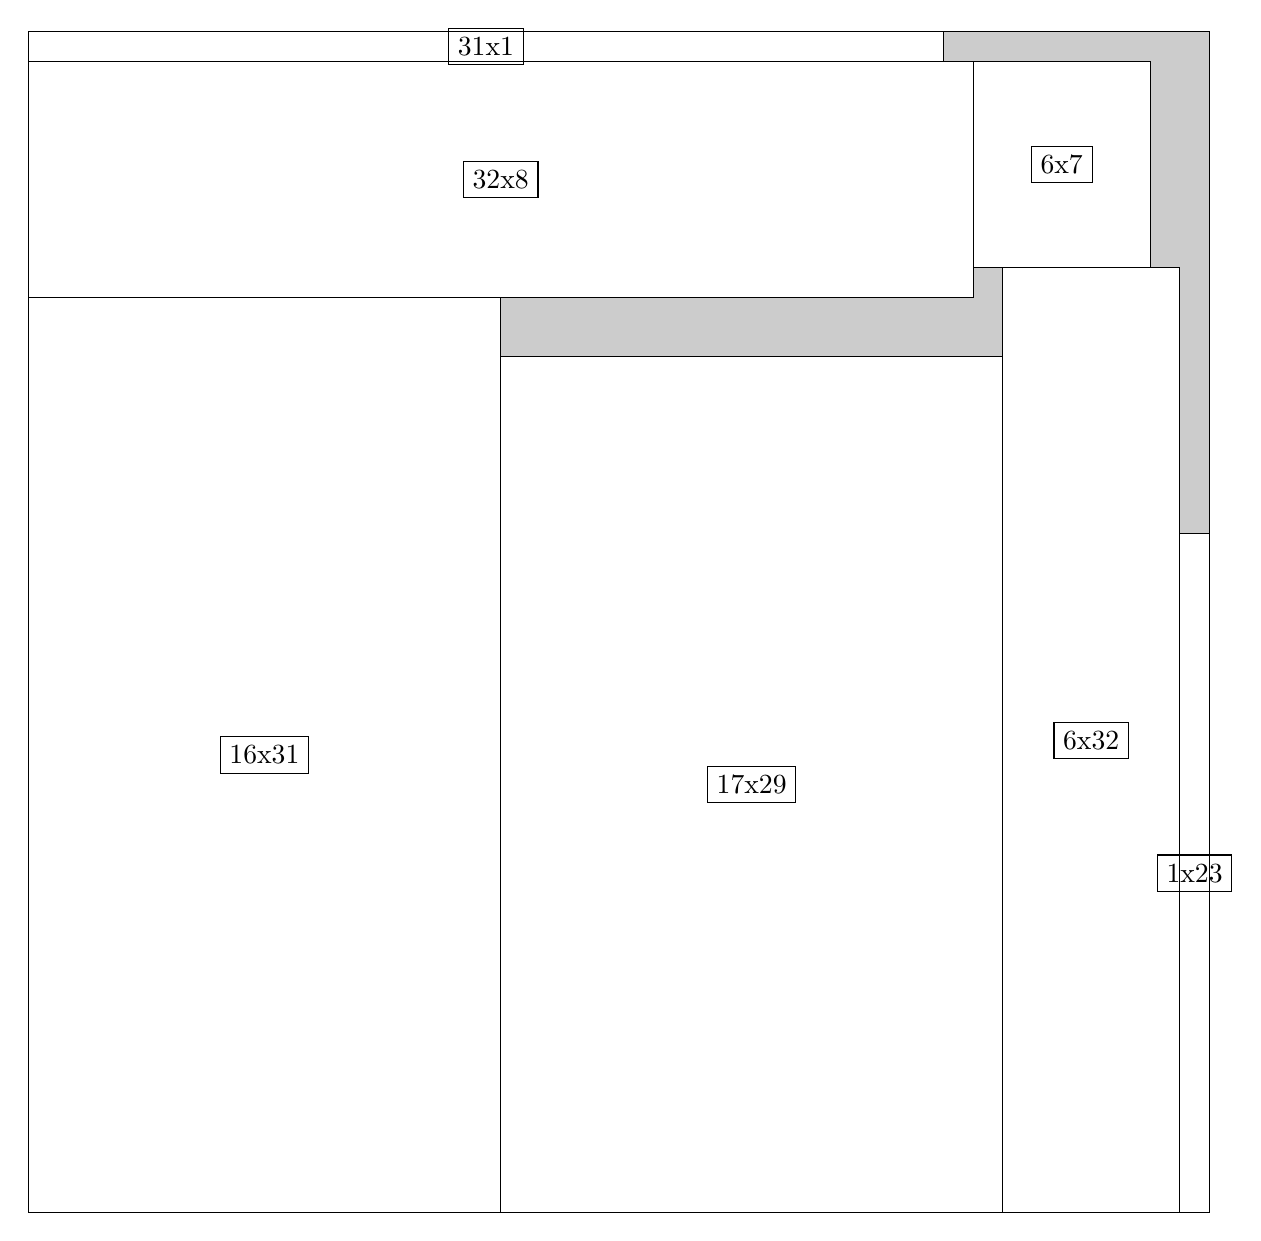
\begin{tikzpicture}[shorten >=1pt,scale=1.0,every node/.style={scale=1.0},->]
\tikzstyle{vertex}=[circle,fill=black!25,minimum size=14pt,inner sep=0pt]
\filldraw[fill=gray!40!white, draw=black] (0,0) rectangle (15.0,15.0);
\foreach \name/\x/\y/\w/\h in {16x31/0.0/0.0/6.0/11.625,17x29/6.0/0.0/6.375/10.875,32x8/0.0/11.625/12.0/3.0,6x32/12.375/0.0/2.25/12.0,6x7/12.0/12.0/2.25/2.625,31x1/0.0/14.625/11.625/0.375,1x23/14.625/0.0/0.375/8.625}
\filldraw[fill=white!40!white, draw=black] (\x,\y) rectangle node[draw] (\name) {\name} ++(\w,\h);
\end{tikzpicture}


w =16 , h =31 , x =0 , y =0 , v =496
\par
w =17 , h =29 , x =16 , y =0 , v =493
\par
w =32 , h =8 , x =0 , y =31 , v =256
\par
w =6 , h =32 , x =33 , y =0 , v =192
\par
w =6 , h =7 , x =32 , y =32 , v =42
\par
w =31 , h =1 , x =0 , y =39 , v =31
\par
w =1 , h =23 , x =39 , y =0 , v =23
\par
\newpage


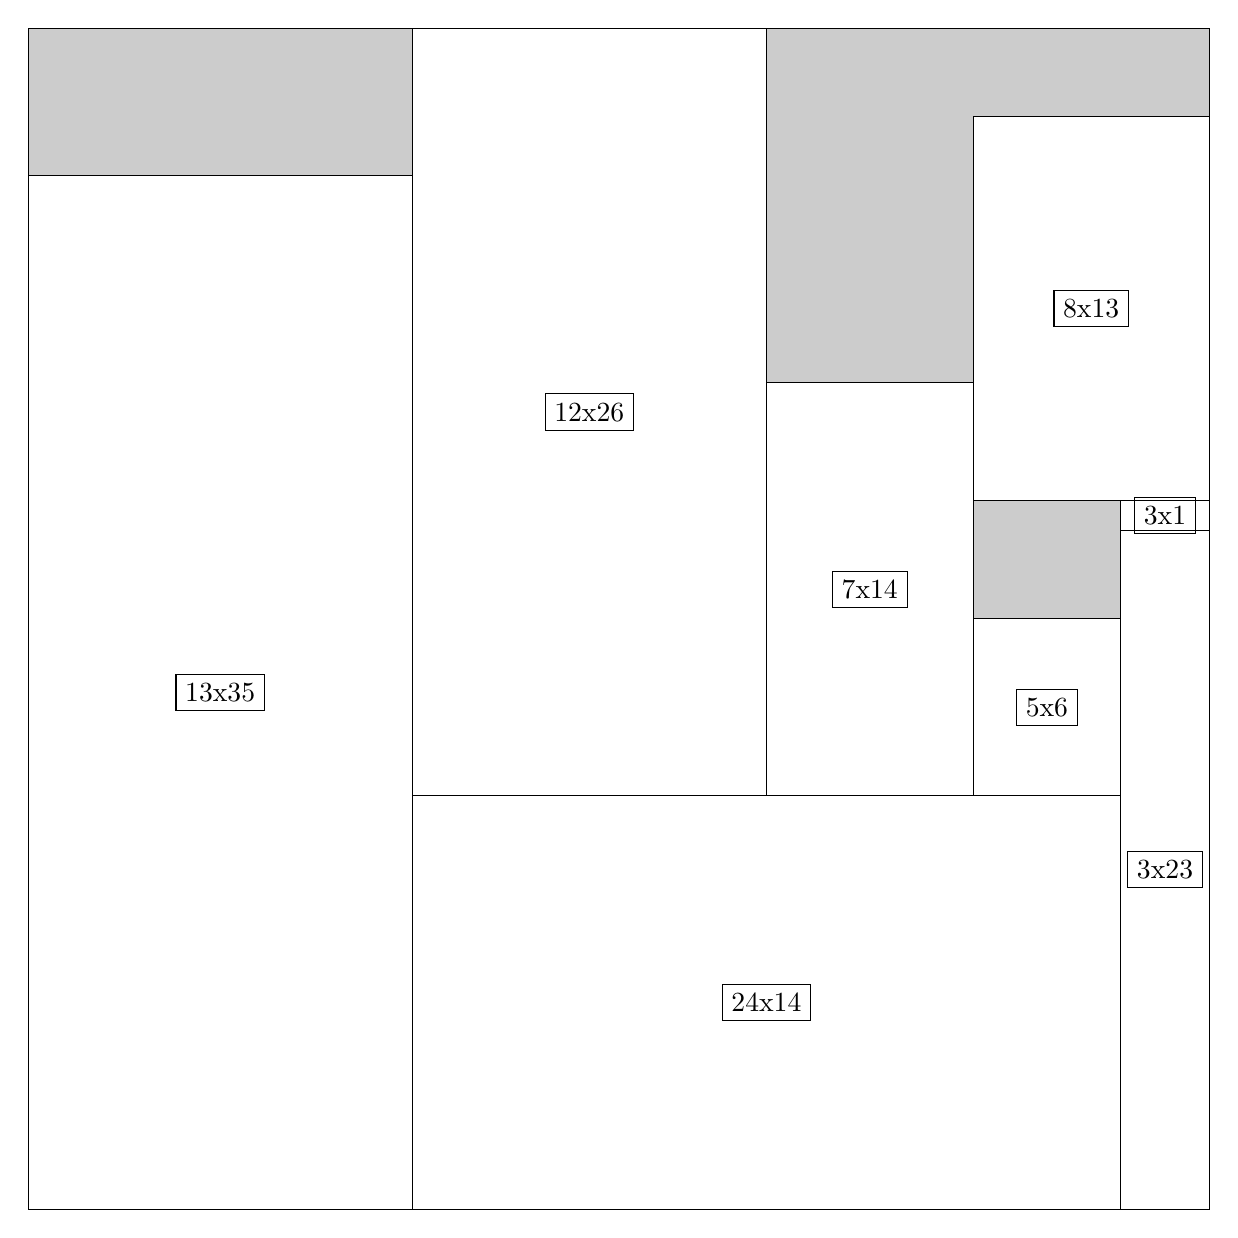
\begin{tikzpicture}[shorten >=1pt,scale=1.0,every node/.style={scale=1.0},->]
\tikzstyle{vertex}=[circle,fill=black!25,minimum size=14pt,inner sep=0pt]
\filldraw[fill=gray!40!white, draw=black] (0,0) rectangle (15.0,15.0);
\foreach \name/\x/\y/\w/\h in {13x35/0.0/0.0/4.875/13.125,24x14/4.875/0.0/9.0/5.25,12x26/4.875/5.25/4.5/9.75,8x13/12.0/9.0/3.0/4.875,7x14/9.375/5.25/2.625/5.25,3x23/13.875/0.0/1.125/8.625,5x6/12.0/5.25/1.875/2.25,3x1/13.875/8.625/1.125/0.375}
\filldraw[fill=white!40!white, draw=black] (\x,\y) rectangle node[draw] (\name) {\name} ++(\w,\h);
\end{tikzpicture}


w =13 , h =35 , x =0 , y =0 , v =455
\par
w =24 , h =14 , x =13 , y =0 , v =336
\par
w =12 , h =26 , x =13 , y =14 , v =312
\par
w =8 , h =13 , x =32 , y =24 , v =104
\par
w =7 , h =14 , x =25 , y =14 , v =98
\par
w =3 , h =23 , x =37 , y =0 , v =69
\par
w =5 , h =6 , x =32 , y =14 , v =30
\par
w =3 , h =1 , x =37 , y =23 , v =3
\par
\newpage


\end{document}